\section{Solution Architecture} \label{sec4}
\noindent
In this section, we explain our solution architecture for schedulability assessment. As described in the previous section, we are given a set of $n$ control loops, with their bus access states marked as the accepting ones. Recall that our scheduling objective is to be able to grant bus access infinitely often to each control loop. To check if the system is safe and schedulable, we carry out the following steps: 

\begin{itemize}

\item We compute the product of the individual control loops using the construction explained below. 

\item Once the product is computed, we look for the presence of a cycle that contains at least one state from each control loop. In other words, on any infinite run of the product automaton, each control loop repeats infinitely often and is therefore, granted bus access infinitely often as well. 

\end{itemize}


\subsection{Intersection Automaton construction}
\noindent
Given a collection of control loops, each expressed as B\"{u}chi automatons, we describe below the methodology for computing their product~\cite{DBLP:books/ws/automata2012/ChevalierDMP12}, which is an important step in our work. For the sake of simplicity and ease of illustration, we explain the product construction in terms of two automatons. 
Let us consider the two B\"{u}chi automatons P and Q, as shown in Fig \ref{fig1} and defined by the
conventional five tuple:

$P = \{(p_0,p_1),(a,b),p_0, Q \times \sum \rightarrow Q,p_1\}$

$Q = \{(q_0,q_1),(a,b),q_0, Q \times \sum \rightarrow Q,q_1\}$


\noindent
We go through the 
following steps for the intersection. 
The classical product on the given input automatons is first constructed. Consider the resulting product automata, starting from the start state. Only the reachable states are considered, as shown in Fig\ref{product}.

\begin{figure}
\begin{center}
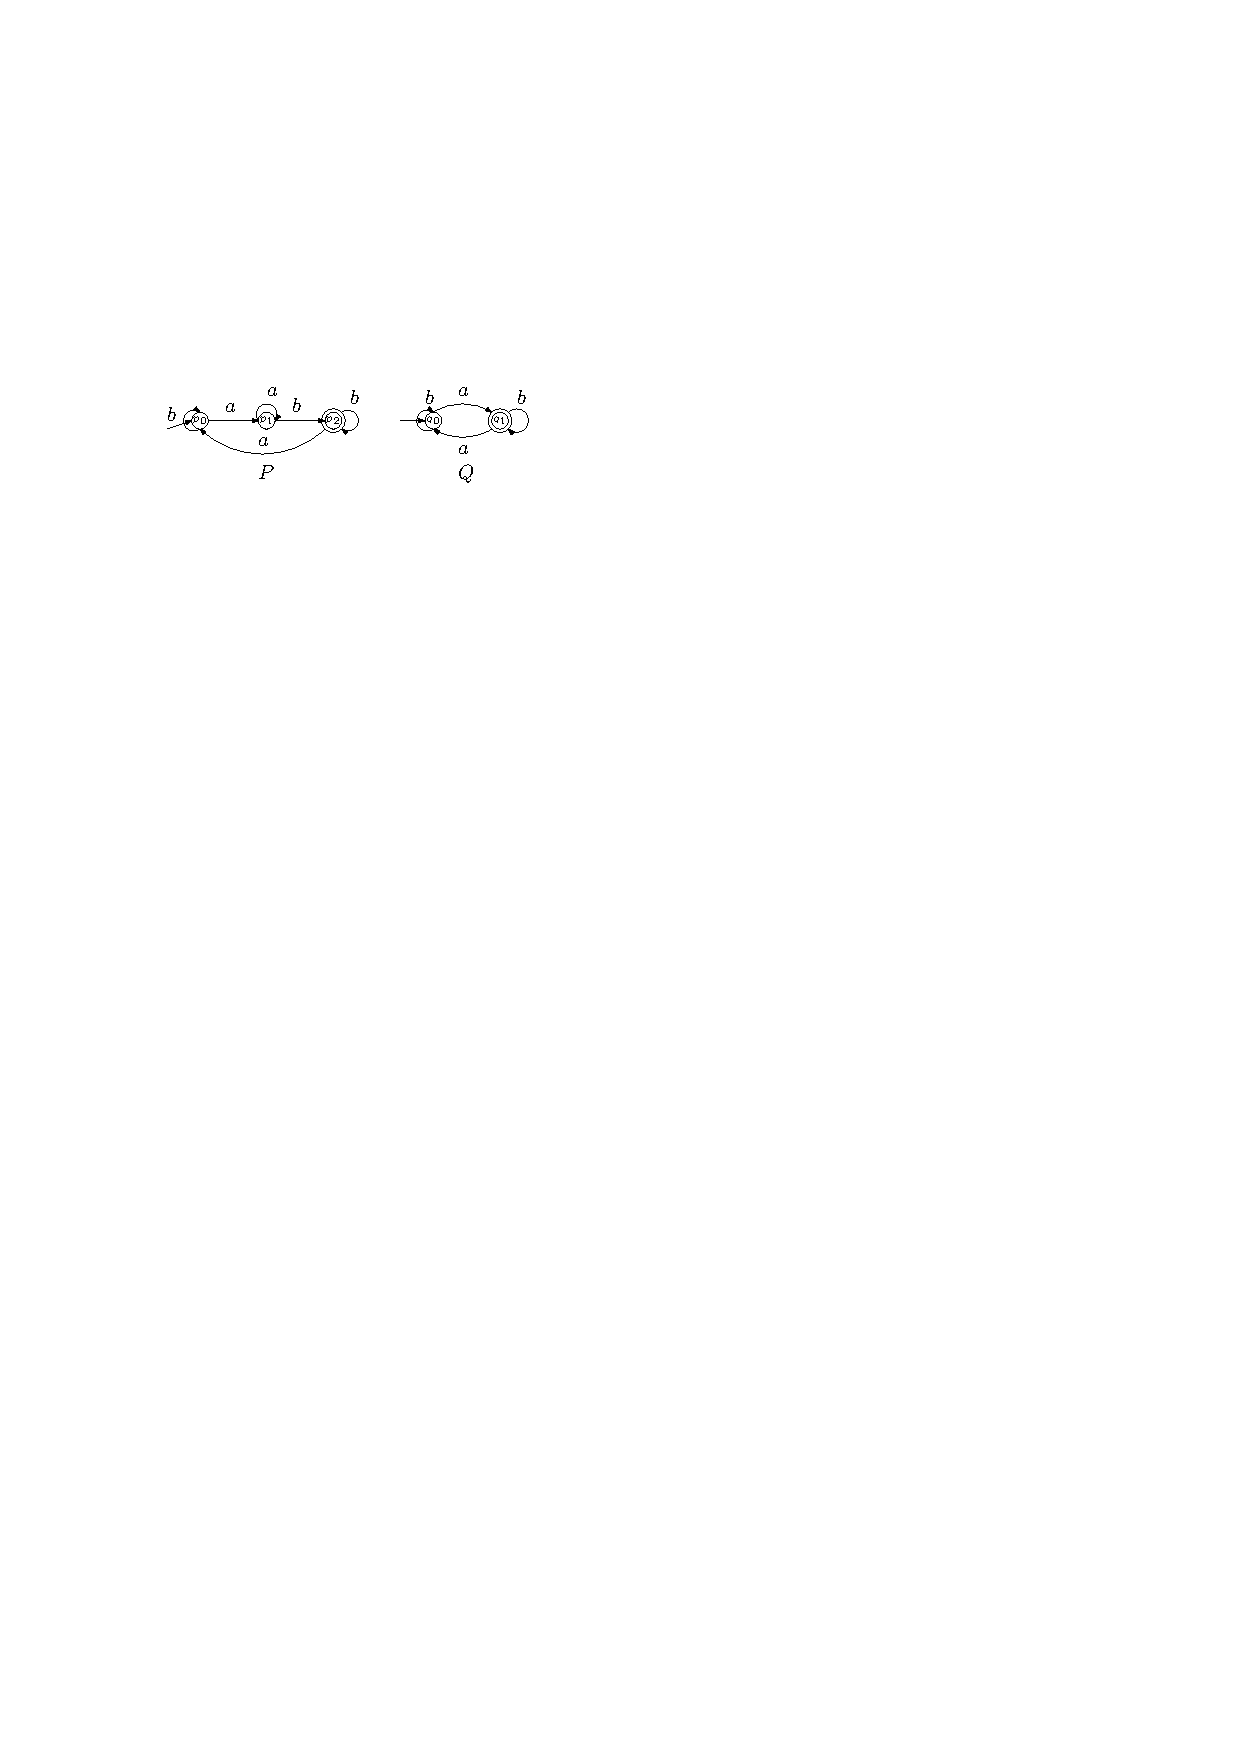
\includegraphics[width=60mm]{example_1.pdf}
\end{center}
%\vspace{-0.1in}
\caption{{\em Individual automatons}} \label{fig1}
\end{figure}

 \begin{figure}
\begin{center}
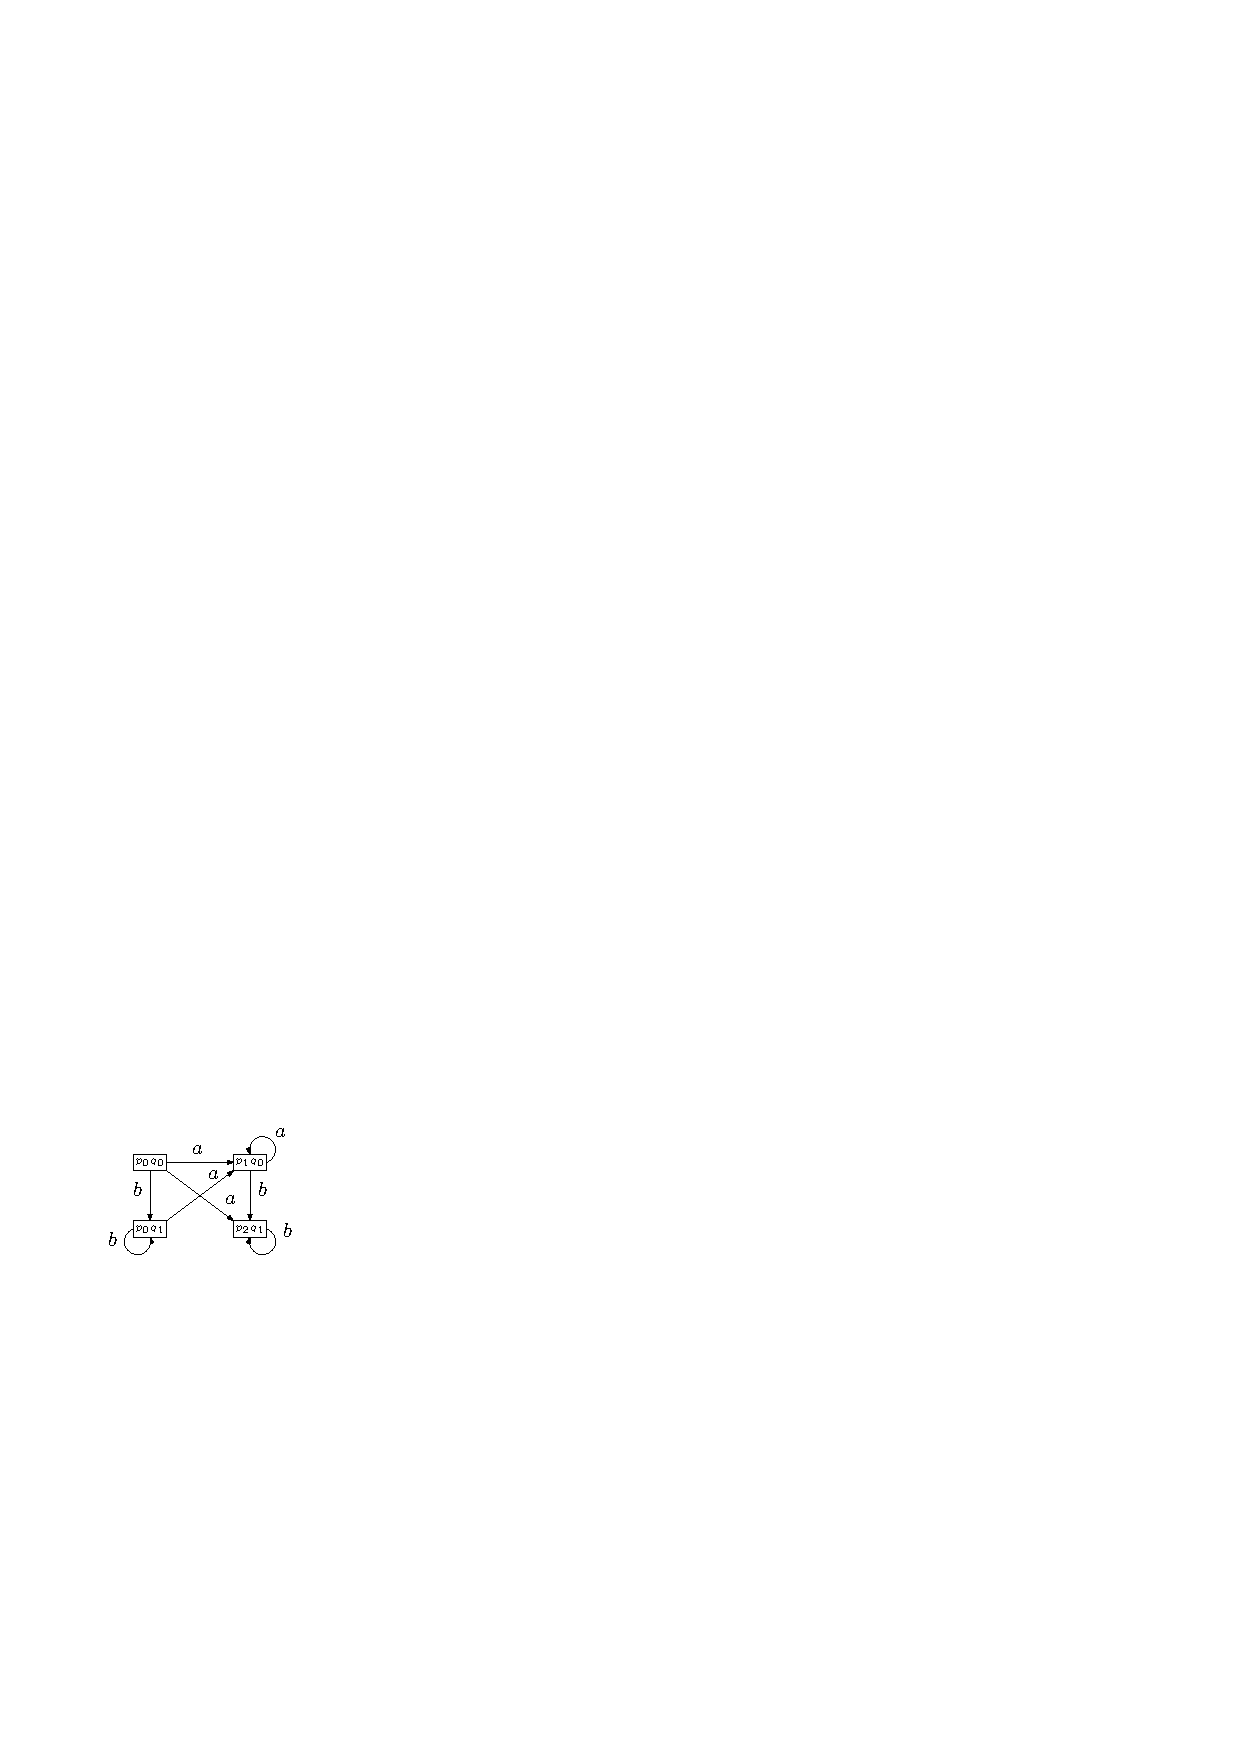
\includegraphics[width=50mm]{product.pdf}
\end{center}
%\vspace{-0.1in}
\caption{{\em Intersection of the input automata}}
\label{product}
\end{figure}
 
~\\
\noindent
Intersection of B\"{u}chi automatons require a special handling to model the infinitary acceptance condition on top of the classical product construction of finite automatons. We can see in Fig~\ref{product} that the states do not contain the tuple $<p_2,q_0>$, the set of final states
 from both the automata. In
 the following steps, we modify the product construction to include accepting states from
 both the automata. The resulting intersection automata ensures that accepting states of both the automatons are visited  infinitely often. From the set of states of each individual automaton, where each state is reachable from the 
 start state, we make three copies of the product automata. In general, for $n$ such automatons, $n$+$1$ copies are made.
 Each copy has a flag with the states, as shown in Fig\ref{fig:copy}. The flags associated with 
 the states are waiting to see the acceptance of the automaton.
In Fig \ref{fig:copy}, flag $1$ is waiting to see the acceptance state of P, flag $2$ is waiting to see
the acceptance state of Q, and states with flag $3$ signify that the track has traversed all the accepting states
of both the automatons. Starting from the first copy, the transitions are made according to the product automaton.
 A transition goes to the next flag if it gets the final state of one automaton. In general, for an automaton state associated with this flag in the product, if the acceptance condition of an automaton is obtained, the transition goes to the next copy, otherwise it remains within the transitions on its own states, as shown in  Fig\ref{transition}. When it reaches the last copy, it has traversed the accepting state of
 each individual automaton. The red cycle in Fig~\ref{transition} shows one such cycle. After reaching the last state, it goes to the first state. In the resulting automaton, a cycle is accepted, when it passes through the last copy
 of the product automaton, that signifies the run of the cycle traverses the accepting states of each automaton infinitely often. The remaining cycles, which do not pass through the last copy, are not accepted. We thus augment the classical product construction for finite automatons to model our infinitary acceptance requirement.
 
  \begin{figure}
\begin{center}
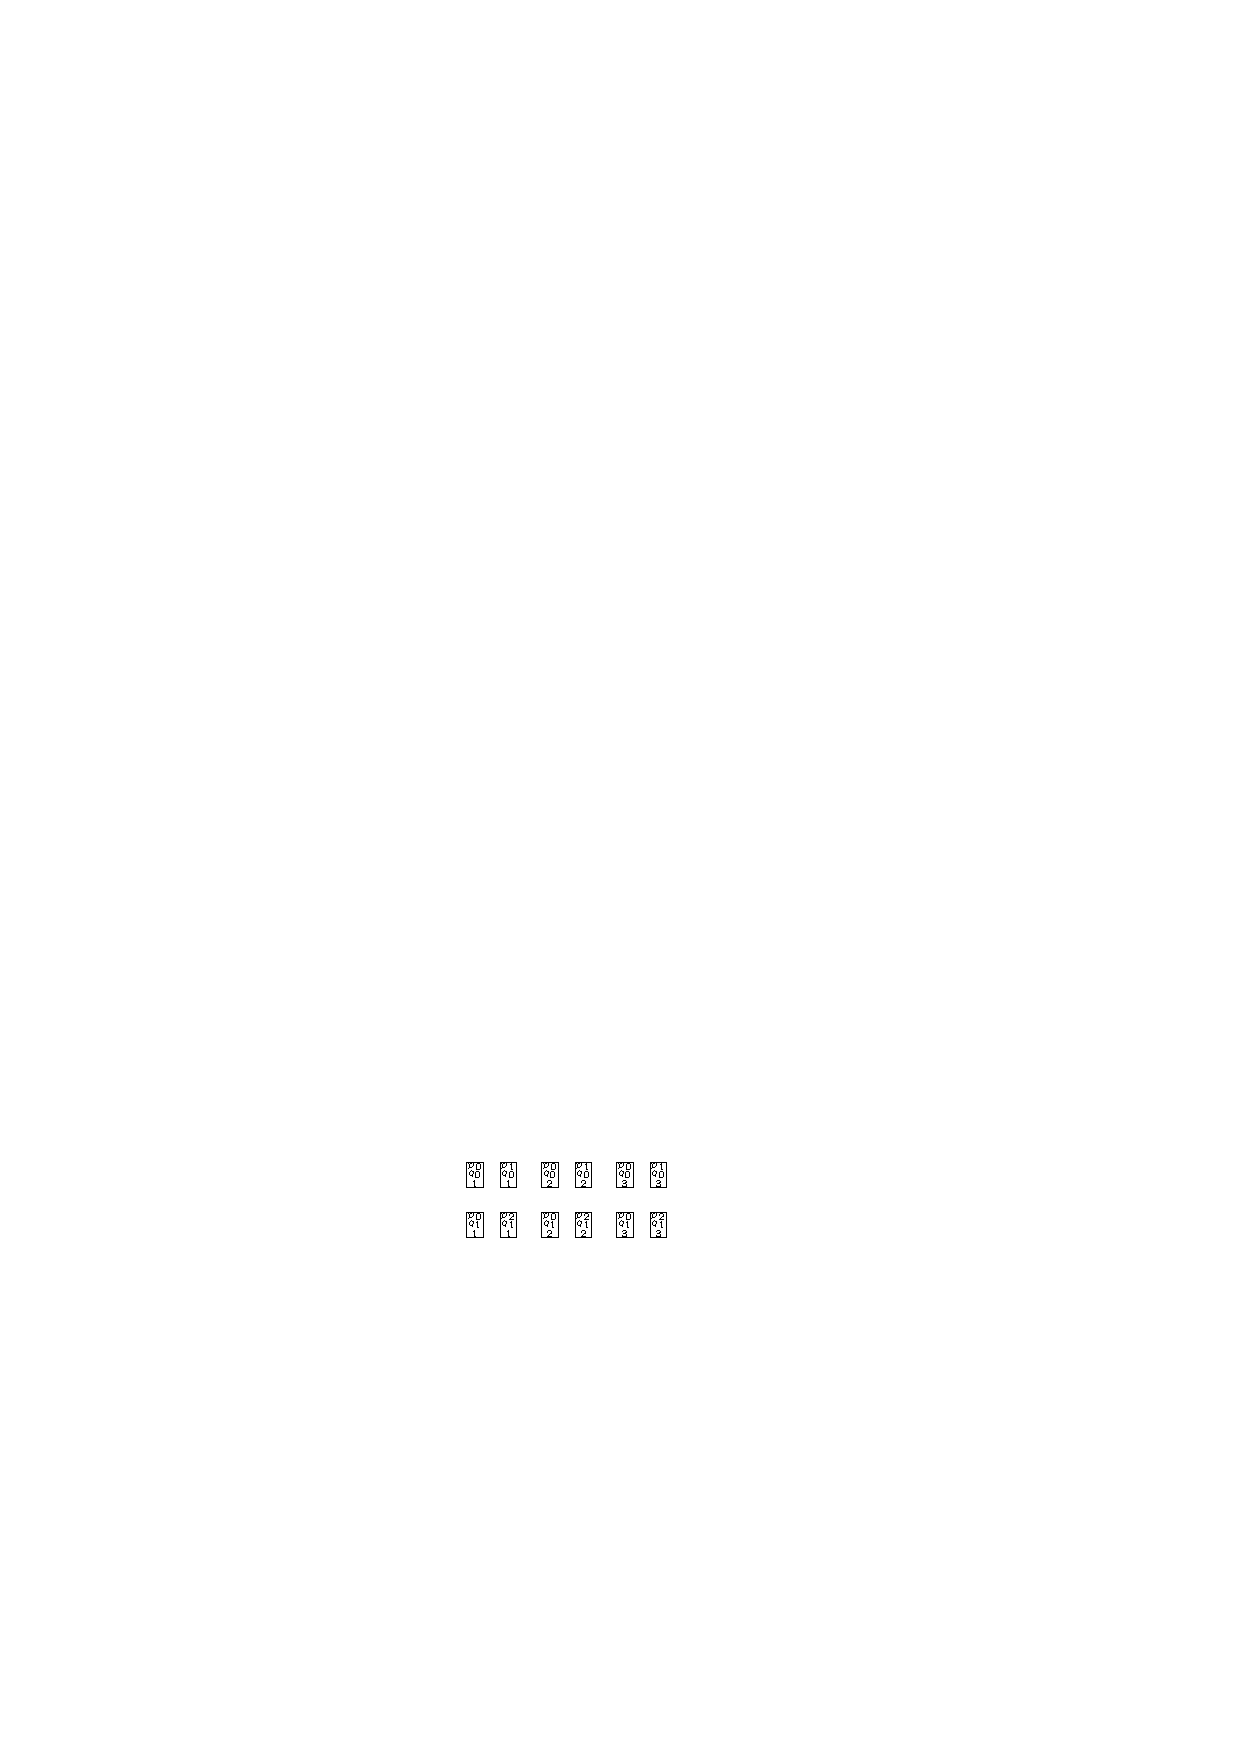
\includegraphics[width=50mm]{state_copy.pdf}
\end{center}
%\vspace{-0.1in}
\caption{{\em Product automata construction with flags}}
\label{fig:copy}
\end{figure}

 
 \begin{figure}
\begin{center}
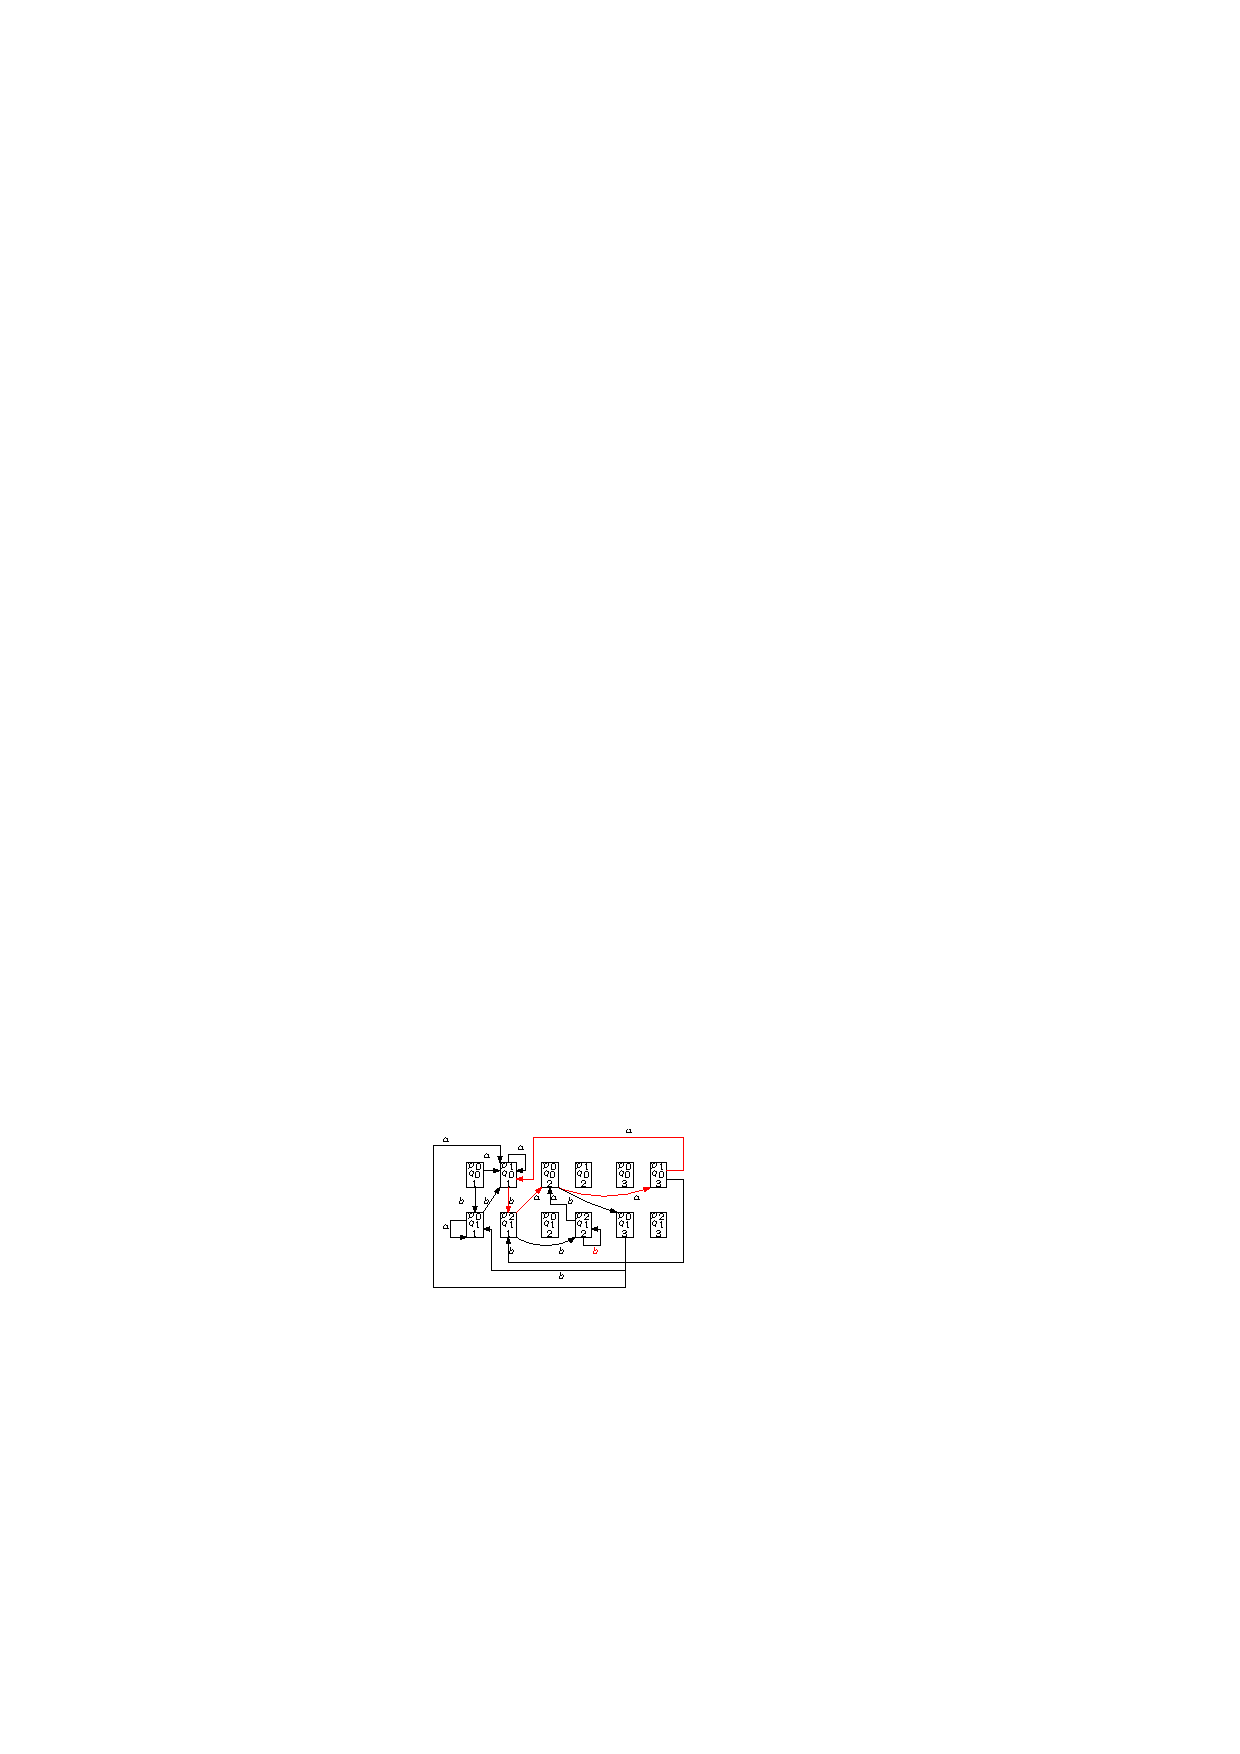
\includegraphics[width=50mm]{state_copy_transition.pdf}
\end{center}
%\vspace{-0.1in}
\caption{{\em Intersection of the input automata}}
\label{transition}
\end{figure}

\begin{figure}
\begin{center}
%\includegraphics[width=50mm, height=75mm]{algorithn.pdf}
\end{center}
%\vspace{-0.1in}
%\caption{{\em Flow chart of our idea}}
\label{fig:Algorithm}
\end{figure}

\subsection{Verifying the scheduling objective}
\noindent
Once the intersection automaton is constructed, the task of looking for cycles starting from the initial states is carried out. Cycle detection algorithms are standard in literature~\cite{Clarke:2000:MC:332656} and we implement the same for this work as well. Once a cycle is found, we traverse the cycle (every cycle is bound to contain a finite number of states) and check if each control loop is represented inside it. If not, we proceed to the next cycle and carry out the same check. If all cycles are exhausted and we do not encounter any one which meets our scheduling objective, we conclude that the schedulability requirement is not met. This step is thus quite straightforward.

\subsection{Code Replacement attack detection}
\noindent
As the system is monitored over time, newer structures of the control loops emerge and we perform the same computation steps outlined above on the modified structures to check if it remains schedulable even in the presence of the modifications. Our mechanism can thus be used as a continuous monitor to safe-guard against intermittent control attacks. 

~\\
\noindent
At this onset, we would like to admit that our framework can point out code replacement attacks only if schedulability is lost. Once the intersection is computed, we may have 3 different possibilities if schedulability is lost. Assuming that the system was schedulable earlier, we may conclude the system has been attacked if any of the following possibilities are detected. Firstly, we may have an empty intersection automaton now. As a second possibility, the product may still be non-empty but a cycle may not be reachable. Finally, a cycle may be found but it may not contain representative tasks from each control loop. All these are indicators of schedulability loss according to our analysis method and we conclude that a replacement attack is carried out. However if the system still remains schedulable according to our scheduling objective, our framework is unable to flag the attack, even if a code replacement has been carried out.